%
% Sección de clasificación de la criptografía, capítulo de antecedentes.
% Proyecto Lovelace.
%

\subsection{Clasificación de la criptografía}
\label{sec:clasificacion}

La criptografía puede clasificarse de forma histórica en dos categorías,
la criptografía clásica y la criptografía moderna. La criptografía clásica
es aquella que se utilizó desde la antigüedad, teniéndose registro de su
uso desde hace más 4000 años por los egipcios, hasta la mitad del siglo
XX. En esta los métodos utilizados para cifrar eran variados, pero en su
mayoría usaban la transposición y la sustitución, además de que la mayoría
se mantenían en secreto. Mientras que la criptografía moderna es la que
se inició después la publicación de la \textit{Teoría de la información}
por Claude Elwood Shannon\cite{shannon_teoria}, dado que esta sentó las
bases matemáticas para la \gls{gl:criptologia} en general.

Una manera de clasificar es de acuerdo a las técnicas y métodos empleados
para cifrar la información, esta clasificación se puede observar en la
figura \ref{clasificacion_cripto}.

\begin{figure}
  \begin{center}
    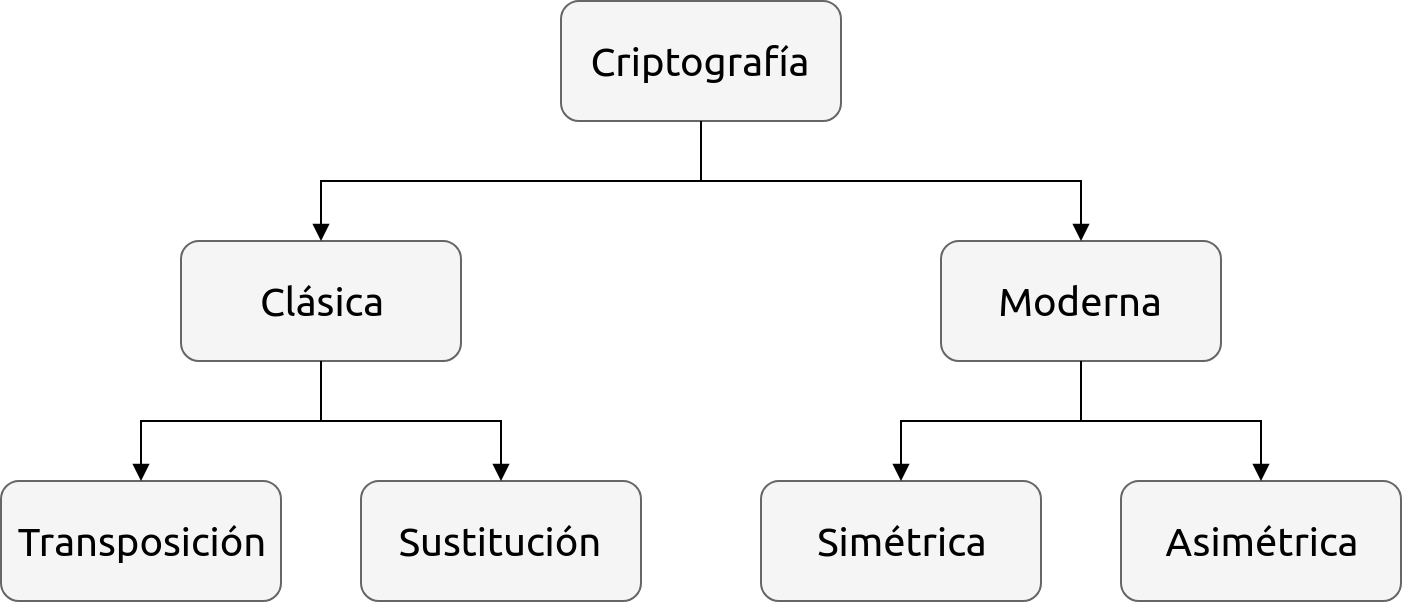
\includegraphics[width=0.75\linewidth]{diagramas/clasificacion_cripto.png}
    \caption{Clasificación de la criptografía.}
    \label{clasificacion_cripto}
  \end{center}
\end{figure}

Adentrándose en la clasificación de la criptografía clásica, se tienen los
cifrados por transposición, los cuales se basan en técnicas de
\gls{gl:permutacion} de forma que los caracteres de la información en claro
se reordenen mediante algoritmos específicos, y los cifrados por sustitución,
que utilizan técnicas de modificación de los caracteres por otros
correspondientes a un alfabeto específico para el cifrado.

En cuanto a la criptografía moderna, esta tiene dos vertientes: la
criptografía simétrica o de llave secreta, y la asimétrica o de llave
pública. Hablando de la primer vertiente, se puede decir que es aquella
que utiliza un modelo matemático para cifrar y descifrar un mensaje
utilizando únicamente una llave que permanece secreta.

\begin{figure}
  \begin{center}
    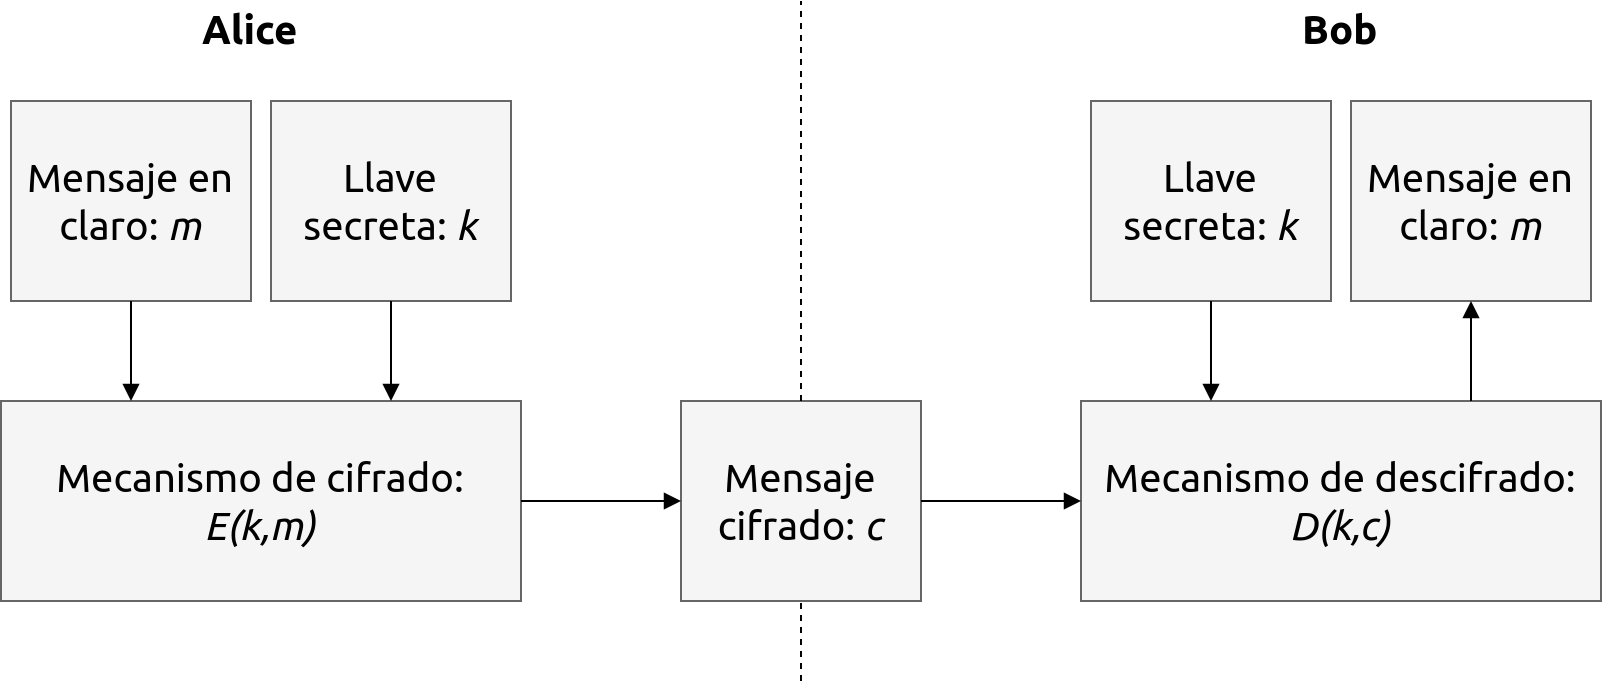
\includegraphics[width=0.8\linewidth]
      {../../../../diagramas_comunes/marco_teorico/cripto_simetrica.png}
    \caption{Canal de comunicación con criptografía simétrica.}
    \label{cripto_simetrica}
  \end{center}
\end{figure}

En la figura \ref{cripto_simetrica} se puede observar el proceso para
establecer una comunicación segura por medio de la criptografía simétrica.
Primero, tanto Alice como Bob deben de establecer una llave única y
compartida $k$, para que después, Alice, actuando como el emisor, cifre un
mensaje $m$ usando la llave $k$ por medio del algoritmo de cifrado $E(k,m)$
para obtener el mensaje cifrado $c$ y enviárselo a Bob. Posteriormente
Bob, como receptor, se encarga de descifrar $c$ con ayuda de la llave $k$
por medio del algoritmo de descifrado $D(k,c)$ para obtener el mensaje original
$m$.

Gran parte de los algoritmos de cifrado que caen en este tipo de criptografía
están basados en las redes Feistel, que son un método de cifrado propuesto
por el criptógrafo Horst Feistel, mismo que desarrolló el \gls{gl:des}
(sección \ref{sec:des}) a principios de la década de los 70, que fue el
cifrado usado por el gobierno estadounidense hasta 2002, año en que el
\gls{gl:aes} (sección \ref{sec:aes}) lo sustituyó.

Ahora, adentrándose en la criptografía asimétrica, se tiene que su idea
principal es el uso de 2 llaves distintas para cada persona, una llave
pública para cifrar, que esté disponible para cualquier otra persona, y una
llave privada para descifrar, que se mantiene disponible solo para su
propietario.

El proceso para establecer una comunicación segura por medio de este tipo
de criptografía es el siguiente: primero, Alice nuevamente como el emisor,
cifra un mensaje $m$ con la llave pública de Bob $pk$, y usa el algoritmo de
cifrado $E(pk,m)$ para obtener $c$ y enviarlo. Después Bob como receptor,
se encarga de descifrar $c$ por medio del algoritmo de descifrado
$D(sk,c)$ haciendo uso de su llave privada $sk$. Este proceso se refleja
gráficamente el la figura \ref{cripto_asimetrica}.

\begin{figure}
  \begin{center}
    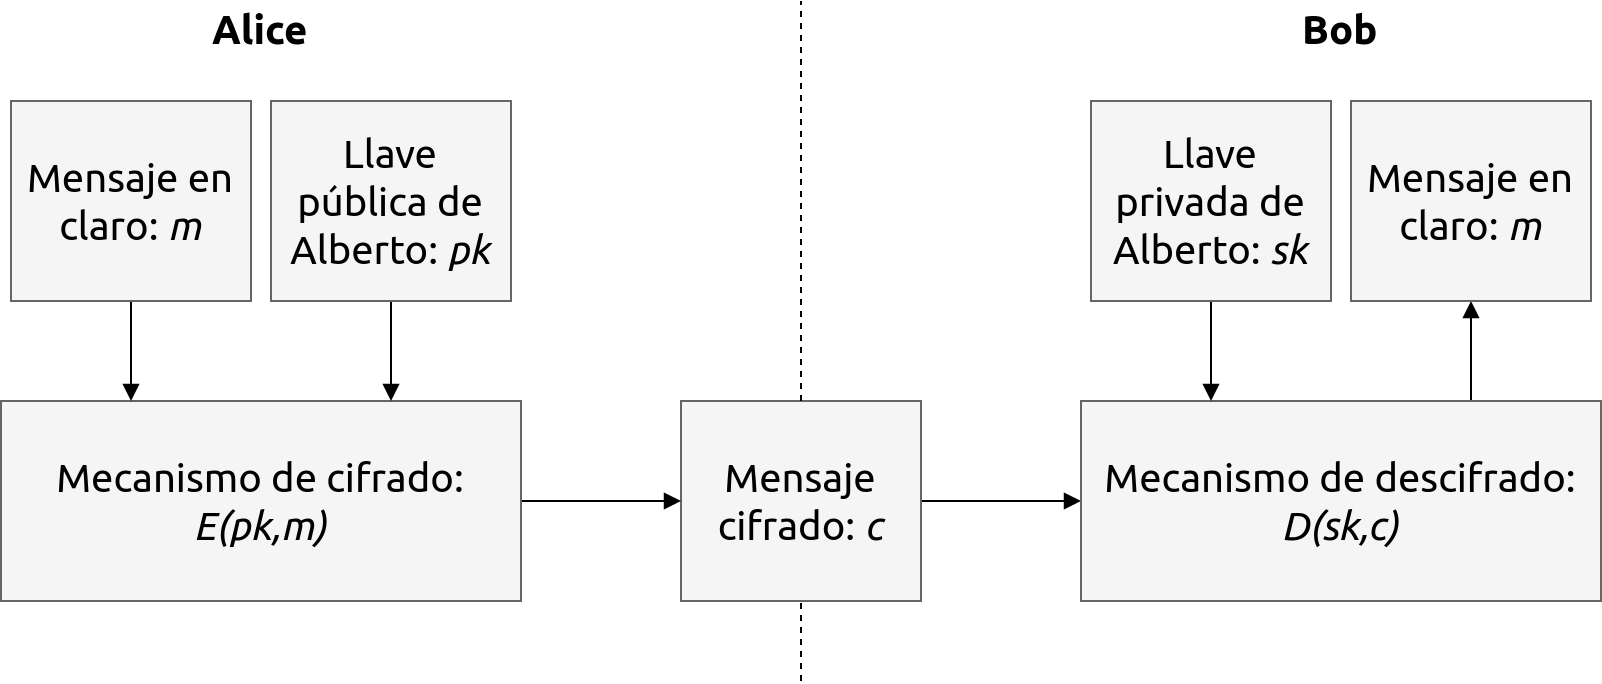
\includegraphics[width=0.8\linewidth]{diagramas/cripto_asimetrica.png}
    \caption{Canal de comunicación con criptografía asimétrica.}
    \label{cripto_asimetrica}
  \end{center}
\end{figure}

Entre los uso que se le da a esta criptografía está el mantener la
distribución de llaves privadas segura y establecer métodos que garanticen
la autenticación y el no repudio; por ejemplo, en las firmas y
certificados digitales.

% El principal precursor de la criptografía asimétrica fue el método de
% intercambio de llaves de Diffie-Hellman, desarrollado y publicado por
% Whitfield Diffie y Martin Hellman, en 1976 en el artículo \textit{New
% Directions in Cryptography}\cite{diffie_hellman}, siendo la primera
% forma práctica para poder establecer una llave secreta compartida
% entre dos partes sin contacto previo por medio de un canal público
% para intercambiar mensajes.

% Otro precursor fue el sistema criptográfico \gls{gl:rsa} (nombre
% obtenido por las siglas de los apellidos de sus desarrolladores: Ron Rivest,
% Adi Shamir y Leonard Adleman), publicado en 1978\cite{rsa_publicacion} y que
% fue el primer sistema criptográfico capaz de servir tanto para cifrar
% mensajes, como para la implementación de firmas digitales. A pesar de que sus
% orígenes son de ya hace casi cuatro décadas, este sistema aún es uno de los
% más ampliamente usados.

% Entre los motivos del éxito de \gls{gl:rsa} está que su funcionamiento
% se basa en la teoría elemental de números, ya que usa propiedades descritas
% en esta teoría; y en su seguridad, ya que se basa en la incapacidad de poder
% factorizar números grandes de forma eficiente.

% El algoritmo de \gls{gl:rsa} consta de 3 partes, la generación de llaves,
% el cifrado y el descifrado. El proceso para poder generar un par de llaves
% (pública y privada) con \gls{gl:rsa} se muestra en el pseudocódigo
% \ref{rsa:1}.

% % Me pasé de 80 caracteres porque dentro del pseudocódigo me marca el salto
% % de línea en el pdf.
% \begin{pseudocodigo}[caption={Proceso de generación de llaves de
%   \gls{gl:rsa}.}, label={rsa:1}]
%     entrada: ninguna.
%     salida:  llave pública $(n,e)$ y privada $(n,d)$.
%     inicio
%       Elegir de forma aleatoria 2 números primos $p$ y $q$, que sean de gran
%       magnitud y de una longitud parecida.
%       Calcular $n\: =\: p \:\cdot \:q$
%       Calcular $\varphi(n) \:= \:(p-1) \:(q-1)$.
%       Elegir un exponente de cifrado $e$ tal que $e \:< \:\varphi(n)$ y $mcd(e,\varphi(n)) \:= \:1$.
%       Encontrar el exponente de descifrado $d$ tal que $e \cdot d \:\mod \:\varphi(n) \:= \:1$.
%     fin
% \end{pseudocodigo}

% Las funciones de cifrado y descifrado, están definidas en las ecuaciones
% \ref{funcion_cifrado_rsa} y \ref{funcion_descifrado_rsa} respectivamente,
% y se aplican números enteros o bloques de bits, siendo funciones biyectivas
% e inversas entre sí.
% \begin{align}
%   \label{funcion_cifrado_rsa}
%   E: \mathbb{Z}_n \longrightarrow \mathbb{Z}_n, x \longmapsto x^e \\
%   \label{funcion_descifrado_rsa}
%   D: \mathbb{Z}_n \longrightarrow \mathbb{Z}_n, x \longmapsto x^d
% \end{align}
